\documentclass{article}
\usepackage[T1]{fontenc}
\usepackage{lmodern}
\usepackage{graphicx}
\usepackage{amsmath,amssymb}
\usepackage[a4paper,margin=2cm]{geometry}
\usepackage[absolute,overlay]{textpos}
\setlength{\TPHorizModule}{1mm}
\setlength{\TPVertModule}{1mm}
\usepackage[indonesian]{babel}
\usepackage{hyperref}
\setlength{\emergencystretch}{2em}
% unit: Halaman 72

\begin{document}

% === Halaman 72 (llm) ===

\begin{center}
\Huge \textcolor{yellow}{Encryption} Is Not \\
\Huge Encoding, Hashing, or Tokenization
\end{center}

\vspace{60mm}

\begin{center}
\fbox{\parbox{0.9\textwidth}{\textbf{Professional habit: define the exact protection goal before choosing the cryptographic primitive.}}}
\end{center}

\vspace{5mm}

Sumber gambar: Slide kuliah tamu dari Burman Noviansyah

% deskripsi: Infografis perbandingan antara Encoding, Hashing, Encryption, Tokenization, dan Signature yang mencakup definisi, contoh algoritma, dan tujuan utamanya.
% bbox normalisasi: [0.0900, 0.3500, 0.9100, 0.6100]
\begin{textblock*}{172.20mm}(18.90mm,103.95mm)
\noindent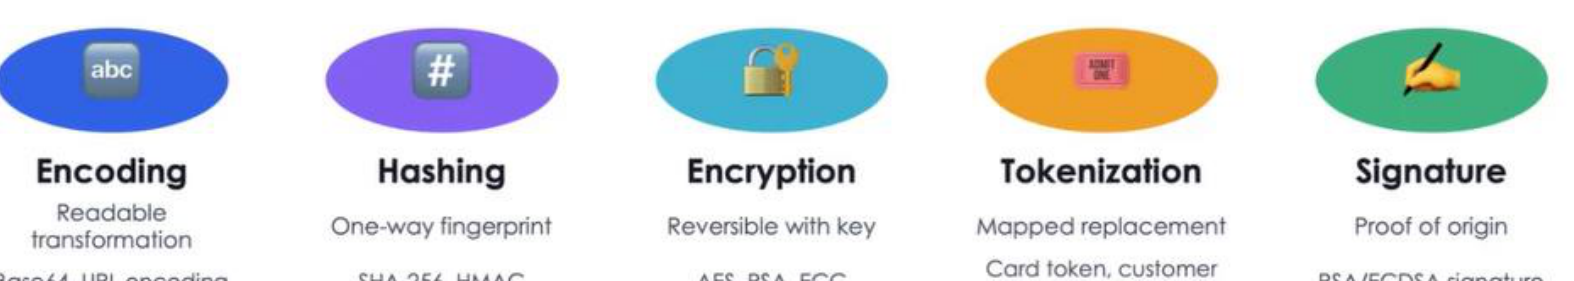
\includegraphics[width=172.20mm,height=77.22mm]{../../images/llm/page_072_img_01.png}%
\end{textblock*}

\end{document}
